\section{Related Works --- FlowBlaze}
\sepframe[image={
\includegraphics[width=3.5cm]{nyu-brand/nyu-torch.jpg}}]

\begin{frame}{Background}
    FlowBlaze~\footfullcite{flowblaze} is an abstration that allows network operators to deploy stateful network functions.

    \begin{itemize}
        \item Implementations exist on the NetFPGA and in software
        \item An extension of RMT (reconfigurable match tables)~\footfullcite{rmt} for stateful processing
    \end{itemize}

    \includegraphics[trim={0.75in 8.35in 0.75in 0.75in}, clip, page=4, width=0.5\linewidth]{assets/rmt.pdf}

    These network functions are focused on operating over packet headers.

    \begin{itemize}
        \item Pipeline starts with parser for packet header fields
        \item A match table operating on these fields determines the next action
        \item Multiple match-actions stages allow later stages to depend on earlier stages
    \end{itemize}

\end{frame}

\begin{frame}{Overview}
    FlowBlaze extends the RMT architecture to support stateful processing within a flow.

    \begin{itemize}
        \item Pipeline contains a series of stateless and stateful stages called ``elements.''
        \begin{itemize}
            \item Stateless elements are similar to RMT match-action stages
        \end{itemize}
    \end{itemize}

    \includegraphics[trim={4.25in 7.40in 0.75in 1.9in}, clip, page=5, width=0.3\linewidth]{assets/flowblaze.pdf}

    \begin{itemize}
        \item Per-flow state is handled using the flow context table, global state using the global registers
        \begin{itemize}
            \item Flow context table is keyed using a list of header fields
            \item Match table replaced with EFSM table, matches on packet fields and flow context
        \end{itemize}
        \item In addition to the action block, an update functions block is added
        \begin{itemize}
            \item Both can also use flow context and global registers as inputs
        \end{itemize}
    \end{itemize}
\end{frame}